\documentclass{beamer}
\mode<presentation>
\usetheme{metropolis} 				% Use metropolis theme
\usepackage[sfdefault]{FiraSans} 	% option 'sfdefault' activates Fira Sans as the default text font				
\usefonttheme{professionalfonts} 	% required for mathspec
\usepackage{pgfpages}
\usepackage{amsmath}
\usepackage{mathtools}
\usepackage{anyfontsize}
\usepackage{circuitikz}
\usepackage{mathptmx}
\usepackage{mathpazo}
\usepackage{xcolor}
\usepackage{pgfplotstable}
\usepackage[breakable]{tcolorbox}
\usepackage{appendixnumberbeamer}
\usepackage[scale=2]{ccicons}
\usepackage{totcount}
\usepackage{graphicx}
\usepackage{cancel}
\usepackage{soul}
\usepackage{tabularx}
\usepackage{fancyvrb}
\usepackage{tikz}
\usepackage{pgfplots}
\usepackage{makeidx}
\usepackage{verbatim}
\usepackage[babel]{csquotes}
\usepackage{caption}
\usepackage{array}
\usepackage{cmap}
\usepackage{subfig}
\usepackage{grffile}
\usepackage{trace}
\usepackage{bookmark}
\usepackage{listings}
\usepackage{scalerel}
\usepackage{hyperref}
\usepackage{parskip}
\usepackage{enumerate}
\usepackage{enumitem}
\usepackage{etex}
\usepackage[etex=true, export]{adjustbox}
\newlength\mylength
\usepackage{neuralnetwork}
\usepackage{appendixnumberbeamer}
\usepackage{relsize}
\usepackage{multicol}
\usepackage{booktabs}
\usepackage{etoolbox}
\usepackage{longtable}
\usepackage[normalem]{ulem}
\usepackage{latexsym}
\usepackage[11pt]{moresize}
\usepackage[mathrm=sym]{unicode-math}
\usepackage{collcell}

\setbeameroption{show notes on second screen}

\setmathfont{FiraMath-Regular.otf}
\setmathfont[range={\vdots,\ddots}]{Asana-Math}
\newcommand*{\MinNumber}{0}%
\newcommand*{\MaxNumber}{1}

\makeatletter
\define@key{adjbox}{settototalheight}[1]{%
    \Gin@esetsize
    \@tempswatrue
    \adjust@addcode{\@collectbox{\global#1=\totalheight\relax\BOXCONTENT}}{}%
}
\makeatother

\DeclarePairedDelimiter\ceil{\lceil}{\rceil}
\DeclarePairedDelimiter\floor{\lfloor}{\rfloor}

\newcommand{\ctikzlabel}[2]{\pbox{\textwidth}{#1\\#2}} % multiple-lines labels
\tikzset{
    pin/.style = {font = \relsize{-2}} % pin font size
}
\ctikzset{
    bipoles/length = 2em, % bipole size
    font = \relsize{-1}, % default font size
}

\adjustboxset{max size={0.9\linewidth}{0.9\paperheight}}
\hypersetup{
	pdftitle={Neural-Networks},
	pdfauthor={Karatzas Andreas},
	bookmarksnumbered=true,
	bookmarksopen=true,
	breaklinks=true,  % so long urls are correctly broken across lines
	urlcolor=urlcolor,
	citecolor=citecolor,
	unicode=true,
	pdfpagemode=FullScreen
}

\DeclarePairedDelimiter\abs{\lvert}{\rvert}

\DeclareCaptionFormat{listing}{\rule{\dimexpr\textwidth+17pt\relax}{0.4pt}\par\vskip1pt#1#2#3}
\captionsetup[lstlisting]{format=listing,singlelinecheck=false, margin=0pt, font={sf},labelsep=space,labelfont=bf}
\renewcommand\lstlistingname{Code}

\newenvironment{fname}{\fontfamily{lmtt}\selectfont}{\par}
\DeclareTextFontCommand{\filename}{\fname}

\hyphenpenalty=1000
\emergencystretch=5em

% Colors for the hyperref package
\definecolor{urlcolor}{HTML}{f25aad}
\definecolor{citecolor}{HTML}{fb5159}

% Colors for the presentation
\definecolor{frametitle-background}{HTML}{1a1a1a}
\definecolor{background-canvas}{HTML}{2c2c2c}
\definecolor{text-f}{HTML}{A3B8CC}
\definecolor{bg-progress-bar}{HTML}{af4747}
\definecolor{fg-progress-bar}{HTML}{d1b08a}
\definecolor{first-fg-block}{HTML}{68a6ee}		% ΜΠΛΕ
\definecolor{second-fg-block}{HTML}{ff8800}		% ΠΟΡΤΟΚΑΛΙ
\definecolor{third-fg-block}{HTML}{5ca382}		% ΠΡΑΣΙΝΟ
\definecolor{fourth-fg-block}{HTML}{8f84ee}		% ΜΩΒ
\definecolor{bg-block}{HTML}{1a1a1a}
\definecolor{title-block}{HTML}{000000}
\definecolor{math-mode}{HTML}{53c5d4}
\definecolor{emph-color}{HTML}{537385}

\metroset{sectionpage=progressbar, progressbar=frametitle, block=transparent, background=dark}

\makeatletter
\setlength{\metropolis@progressinheadfoot@linewidth}{1pt}
\setlength{\metropolis@titleseparator@linewidth}{1pt}
\setlength{\metropolis@progressonsectionpage@linewidth}{1.5pt}

\setbeamertemplate{progress bar in section page}{
  \setlength{\metropolis@progressonsectionpage}{%
    \textwidth * \ratio{\thesection pt}{\totvalue{totalsection} pt}%
  }%
  \begin{tikzpicture}
    \fill[bg] (0,0) rectangle (\textwidth, \metropolis@progressonsectionpage@linewidth);
    \fill[fg] (0,0) rectangle (\metropolis@progressonsectionpage, \metropolis@progressonsectionpage@linewidth);
  \end{tikzpicture}%
}
\makeatother

\newcounter{totalsection}
\regtotcounter{totalsection}

\AtBeginDocument{%
    \pretocmd{\section}{\refstepcounter{totalsection}}{\typeout{Yes, prepending was successful}}{\typeout{No, prepending was not it was successful}}%
}%

\setbeamercolor{titlelike}{parent=normal text, fg=text-f}
\setbeamercolor{background canvas}{bg=background-canvas}
\setbeamercolor{section title}{fg=text-f,bg=text-f}
\setbeamercolor{progress bar}{fg=fg-progress-bar,bg=bg-progress-bar}
\setbeamercolor{normal text}{fg=text-f}
\setbeamercolor{frametitle}{fg=text-f,bg=frametitle-background}
\usebeamercolor[fg]{normal text}


\DeclareMathOperator*{\argmax}{argmax} 		% no space, limits underneath in displays
\DeclareMathOperator*{\argmin}{argmin} 		% no space, limits underneath in displays

\setbeamertemplate{title page}{
	\begin{minipage}[c][\paperheight]{\textwidth}
		\vfill%
		{
			\centering
			\ifx\inserttitle\@empty\else\usebeamertemplate*{title}\fi
			\ifx\insertsubtitle\@empty\else\usebeamertemplate*{subtitle}\fi
		}
		\usebeamertemplate*{title separator}
		\begin{minipage}[t]{.5\textwidth}
			\ifx\beamer@shortauthor\@empty\else\usebeamertemplate*{author}\fi
			\ifx\insertdate\@empty\else\usebeamertemplate*{date}\fi
		\end{minipage}
		\begin{minipage}[t]{.5\textwidth}
			\vspace*{2em}
			{\hspace{1em}\small Instructor: Mohammad Sayeh\par}
			
		\end{minipage}%
	\vspace*{2.0em}
		\begin{minipage}[t]{\textwidth}
			\centering
			\ifx\insertinstitute\@empty\else\usebeamertemplate*{institute}\fi
			\vspace*{-2.5em}
			\ifx\inserttitlegraphic\@empty\else\usebeamertemplate*{title graphic}\fi
		\end{minipage}
		\vfill
		\vspace*{2.5cm}
	\end{minipage}
}

\setbeamertemplate{title}{
	%  \raggedright%  % <-- Comment here
	\linespread{1.0}%
	\inserttitle%
	\par%
	\vspace*{0.5em}
}
\setbeamertemplate{subtitle}{
	%  \raggedright%  % <-- Comment here
	\insertsubtitle%
	\par%
	\vspace*{0.5em}
}

\usetikzlibrary{positioning,fit}

\tikzset{%
   neuron missing/.style={
    draw=none, 
    scale=2,
    text height=0.333cm,
    execute at begin node=\color{text-f}$\vdots$
  },
}

\newcommand{\DrawNeuronalNetwork}[2][]{
\xdef\Xmax{0}
\foreach \Layer/\X/\Col/\Miss/\Lab/\Count/\Content [count=\Y] in {#2}
{\pgfmathsetmacro{\Xmax}{max(\X,\Xmax)}
 \xdef\Xmax{\Xmax}
 \xdef\Ymax{\Y}
}
\foreach \Layer/\X/\Col/\Miss/\Lab/\Count/\Content [count=\Y] in {#2}
{\node[anchor=south] at ({2*\Y},{\Xmax/2+0.1}) {\Layer};
 \foreach \m in {1,...,\X}
 {
  \ifnum\m=\Miss
   \node [neuron missing] (neuron-\Y-\m) at ({2*\Y},{\X/2-\m}) {};
  \else
   \node [circle,fill=\Col!50,minimum size=1cm] (neuron-\Y-\m) at 
  ({2*\Y},{\X/2-\m}) {\Content};
 \ifnum\Y=1
  \else
   \pgfmathtruncatemacro{\LastY}{\Y-1}
   \foreach \Z in {1,...,\LastX}
   {
    \ifnum\Z=\LastMiss
    \else
     \draw[->] (neuron-\LastY-\Z) -- (neuron-\Y-\m);
    \fi
    }
  \fi
 \fi
 \ifnum\Y=1
  \ifnum\m=\X
   \draw [overlay] (neuron-\Y-\m) -- (state);
  \else
   \ifnum\m=\Miss
   \else
    \draw [overlay] (neuron-\Y-\m) -- (state);
   \fi
  \fi
 \else
 \fi     
 }
 \xdef\LastMiss{\Miss}
 \xdef\LastX{\X}
}
}

%%%%%%%%%%%%%%%%%%% Local functions %%%%%%%%%%%%%%%%%%%
%% -- Draw marks
\newbox\dumbox
\newcommand{\mymark}[2]{%
  \setbox\dumbox=\hbox{#2}%
  \hbox to \wd\dumbox{\hss%
    \tikz[overlay,remember picture,baseline=(#1.base)]{ \node (#1) {\box\dumbox}; }%
    \hss}%
}

%% -- Draw small coefficient
\newcommand{\mysmall}[1]{%
  \tikz[overlay,remember picture]{%
    \node[first-fg-block,scale=.5, shift={(0,-.1)}] {x#1};%
  }%
}
%%%%%%%%%%%%%%%%%%% Local functions %%%%%%%%%%%%%%%%%%%

% CHEATING DASH FROM https://tex.stackexchange.com/a/133357/128068
\tikzset{
    cheating dash/.code args={on #1 off #2}{
        % Use csname so catcode of @ doesn't have do be changed.
        \csname tikz@addoption\endcsname{%
            \pgfgetpath\currentpath%
            \pgfprocessround{\currentpath}{\currentpath}%
            \csname pgf@decorate@parsesoftpath\endcsname{\currentpath}{\currentpath}%
            \pgfmathparse{\csname pgf@decorate@totalpathlength\endcsname-#1}\let\rest=\pgfmathresult%
            \pgfmathparse{#1+#2}\let\onoff=\pgfmathresult%
            \pgfmathparse{max(floor(\rest/\onoff), 1)}\let\nfullonoff=\pgfmathresult%
            \pgfmathparse{max((\rest-\onoff*\nfullonoff)/\nfullonoff+#2, #2)}\let\offexpand=\pgfmathresult%
            \pgfsetdash{{#1}{\offexpand}}{0pt}}%
    }
}

\tikzset{
    vertical line/.style args={with style #1 right of column #2 in
    row #3}{
        append after command={
            \pgfextra{ \pgfmathparse{int(#2+1)} 
            \path (\tikzlastnode-#3-#2.east) -- (\tikzlastnode-#3-\pgfmathresult.west) coordinate [midway] (MiloX); 
            \draw [#1] (MiloX |- \tikzlastnode.north) -- (MiloX |- \tikzlastnode.south);
            }
        }
    },
    horizontal line/.style args={with style #1 below row #2 in 
    column #3}{append after command={\pgfextra{ \pgfmathparse{int(#2+1)}
    \path (\tikzlastnode-#2-#3.south) -- (\tikzlastnode-\pgfmathresult-#3.north) coordinate [midway] (MiloY); 
    \draw [#1] (MiloY -| \tikzlastnode.west) -- (MiloY -| \tikzlastnode.east);
    }}
    }
}

\newtoggle{inTableHeader}% Track if still in header of table
\toggletrue{inTableHeader}% Set initial value
\newcommand*{\StartTableHeader}{\global\toggletrue{inTableHeader}}%
\newcommand*{\EndTableHeader}{\global\togglefalse{inTableHeader}}%

% Redefine tabular to initialize \StartTableHeader at start and end
\let\OldTabular\tabular%
\let\OldEndTabular\endtabular%
\renewenvironment{tabular}{\StartTableHeader\OldTabular}{\OldEndTabular\StartTableHeader}%

\newcommand{\ApplyGradient}[1]{%
		\iftoggle{inTableHeader}{#1}{
        \pgfmathsetmacro{\PercentColor}{100.0*(#1-\MinNumber)/(\MaxNumber-\MinNumber)}
        \hspace{-0.33em}\colorbox{white!\PercentColor!frametitle-background}{}}
}
\newcolumntype{R}{>{\collectcell\ApplyGradient}c<{\endcollectcell}}

 
\setlength{\fboxsep}{3mm} % box size

\title{Neural Networks}
\subtitle{Feed Forward Neural Network in C++ 17 and OpenMP for performance optimization}
\date{\today}
\author{Andreas Karatzas}
\institute{Electrical, Computer and Biomedical Engineering}
\titlegraphic{
\includegraphics[scale=.3]{saluki.png}}


\begin{document}

\begin{frame}
	\titlepage
	
	\note{Hello, 
    
    My name is Andreas, and today I'll share with you my work for course ECE 572, "Neural Networks"}
\end{frame}

%%%%%%%%%%%%%%%%%%%% INTRODUCTION %%%%%%%%%%%%%%%%%%%%
\section{Introduction}

\begin{frame}{Abstract}
\begin{tcolorbox}[colback=bg-block,colframe=first-fg-block,coltext=text-f,coltitle=title-block, title=Problem Statement]
Optimizing the performance of a Feed Forward Neural Network.
\end{tcolorbox}
\note{My work for the course's project was on optimizing the performance of a typical Feed Forward Neural Network, alternatively known as Multi-layer Perceptron.}
\end{frame}
\begin{frame}{What}
\begin{adjustbox}{width={\textwidth},totalheight={6cm},keepaspectratio}
\begin{tcolorbox}[colback=bg-block,colframe=third-fg-block,coltext=text-f,coltitle=title-block, title=Overview]
\begin{itemize}
\item[1] Comparison of state-of-the-art deep learning frameworks
\item[2] Implement a neural network application that utilizes all system cores efficiently
\end{itemize}
\end{tcolorbox}
\end{adjustbox}

\note{To really grasp the magnitude of this work, I also implemented the same neural network using PyTorch. Furthermore, I implemented a serial version of my neural network and then I optimized it using a framework called OpenMP.}

\end{frame}

\begin{frame}{Why?}
\begin{figure}
	\centering
    \subfloat[The rise of Deep Learning.\label{fig:deep-learning}]{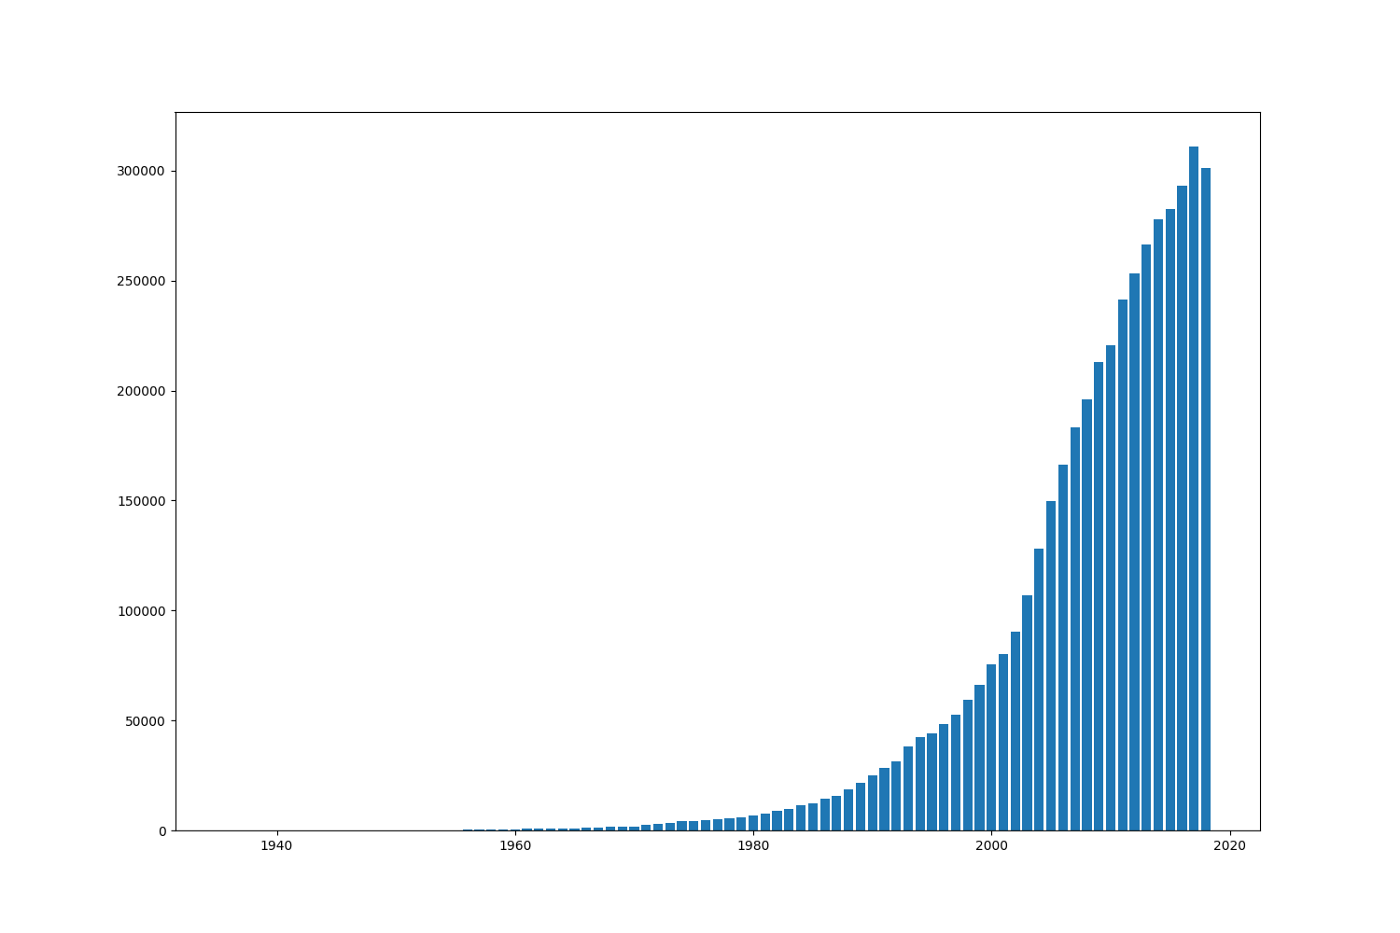
\includegraphics[width=0.4\textwidth, height=0.4\textheight]{deep-learning.png}}\qquad
    \subfloat[The struggle of performance.\label{fig:speed}]{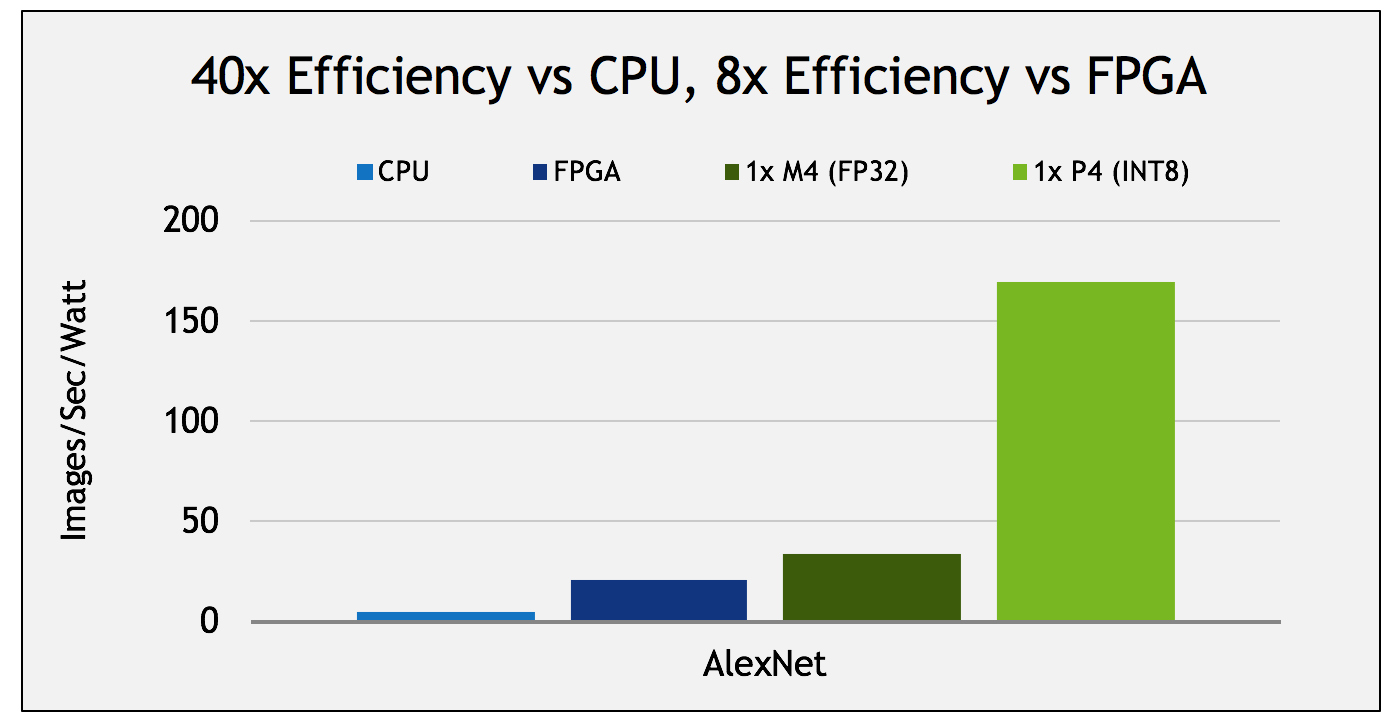
\includegraphics[width=0.4\textwidth, height=0.4\textheight]{speed.png}}
    \caption{Speed is still an issue.}
    \label{fig:performance}
\end{figure}

\note{So why does that work matter? First of all, we live in the era of deep learning. There is an exponential growth on the field of AI and that means that work published in the field of machine learning matters to the research community. Furthermore, performance is and probably will always be a subject for discussion. Let's not forget that the very reason that neural networks did not succeed in dominating the field of computer science was when they first appeared was partially because of limited computational power at that time.}

\end{frame}

\begin{frame}{How?}
\begin{figure}
	\centering
    \subfloat[Multi-core Systems.\label{fig:multicore}]{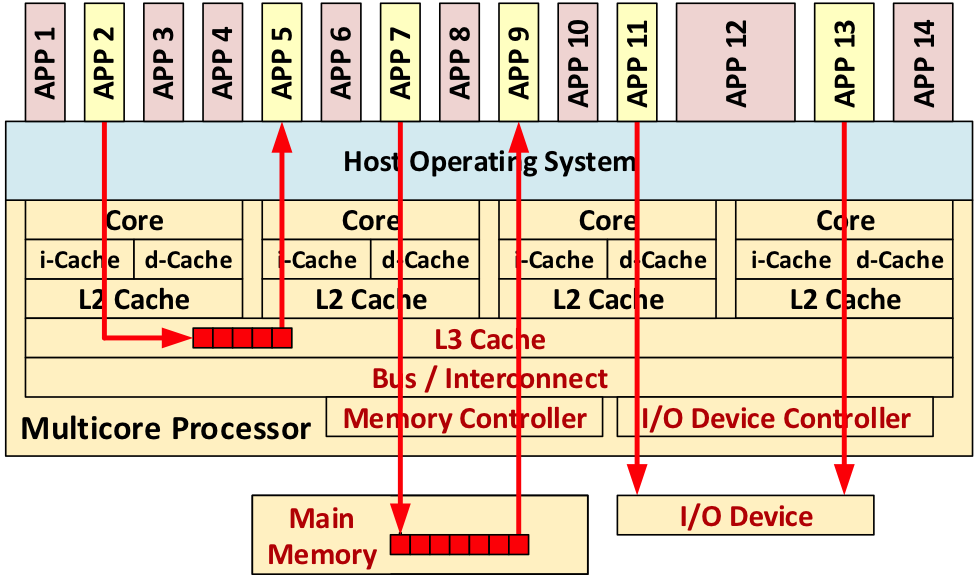
\includegraphics[width=0.4\textwidth, height=0.4\textheight]{multicore.png}}\qquad
    \subfloat[Multi-threading.\label{fig:threading}]{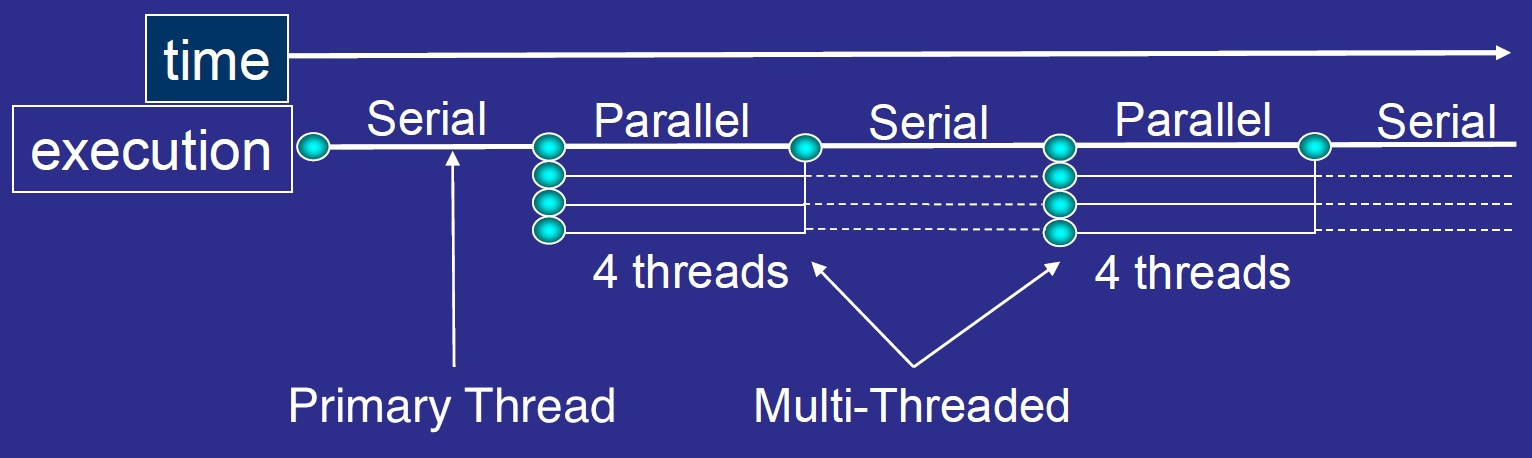
\includegraphics[width=0.4\textwidth, height=0.4\textheight]{forkJoinThreads.png}}
    \caption{Exploiting the hardware using software.}
    \label{fig:how}
\end{figure}

\note{\tiny There are some pretty straight forward ways of optimizing an application. First of all, we have to take into consideration today's general computer system architecture. That is basically the CPU architecture. Today's era regarding CPU architectures is the many-core era. This means that there might be quite a lot of individual cores inside a single chip. Therefore, our goal is how to efficiently utilize all that hardware. However, to beat the state-of-the-art deep learning frameworks, we have to take it to the next level. That is to implement the whole project using low level programming languages, which were created in the first place for performance purposes.}

\end{frame}

%%%%%%%%%%%%%%%%%%%% BACKGROUND %%%%%%%%%%%%%%%%%%%%
\section{Background}

\begin{frame}{Feed Forward Neural Networks}
\begin{figure}
\centering
\def\layersep{2.5cm}
\begin{tikzpicture}[shorten >=1pt,->,draw=black!50, node distance=\layersep]
    \tikzstyle{every pin edge}=[<-,shorten <=1pt]
    \tikzstyle{neuron}=[circle,fill=black!25,minimum size=17pt,inner sep=0pt]
    \tikzstyle{input neuron}=[neuron, fill=bg-progress-bar];
    \tikzstyle{output neuron}=[neuron, fill=first-fg-block];
    \tikzstyle{hidden neuron}=[neuron, fill=second-fg-block];
    \tikzstyle{annot} = [text width=4em, text centered]

    % Draw the input layer nodes
    \foreach \name / \nny in {1,...,3}
    % This is the same as writing \foreach \name / \y in {1/1,2/2,3/3,4/4}
        \node[input neuron] (I-\name) at (0,-\nny) {};

    % Draw the hidden layer nodes
    \foreach \name / \nny in {1,...,4}
        \path[yshift=0.5cm]
            node[hidden neuron] (H-\name) at (\layersep,-\nny cm) {};

    % Draw the output layer node
    \node[output neuron,pin={[pin edge={->}]right:Output}, right of=I-2, xshift=\layersep] (O) {};

    % Connect every node in the input layer with every node in the
    % hidden layer.
    \foreach \source in {1,...,3}
        \foreach \dest in {1,...,4}
            \path (I-\source) edge (H-\dest);

    % Connect every node in the hidden layer with the output layer
    \foreach \source in {1,...,4}
        \path (H-\source) edge (O);

    % Annotate the layers
    \node[annot,above of=H-1, node distance=1cm] (hl) {Hidden layer};
    \node[annot,left of=hl] {Input layer};
    \node[annot,right of=hl] {Output layer};
\end{tikzpicture}
\caption{A typical Feed Forward Neural Network architecture.}
\label{fig:mlp}
\end{figure}

\note{\fontsize{9}{11}\selectfont Let us first study the problem from a high level overview. In this figure, we can see the general layout of a feed forward neural network. We can immediately trace some points where we can reconfigure the execution to run in parallel. For example, since forward propagation is really just a GEMM operation we can split the workload of each neuron to a separate task.}
\end{frame}
\begin{frame}{The Perceptron}
\begin{figure}
\centering
\begin{tikzpicture}[>=latex]
\path
(0,0)     node[circle,draw,scale=2,inner sep=2pt] (S) {$\Sigma$}
+(90:2.5) node[circle,draw,inner sep=2.5pt] (b) {}
          node[above=1mm] {$b^{[j]}$}
+(-3.5,1.5)  node[circle,text=bg-progress-bar,fill=text-f!30]  (x1) {$a_1^{[j - 1]}$}
+(-3.5,0)    node[circle,text=bg-progress-bar,fill=text-f!30]  (x2) {$a_2^{[j - 1]}$}
+(-3.5,-1.5) node[circle,text=bg-progress-bar,fill=text-f!30]  (x3) {$a_3^{[j - 1]}$}
(2,0)    node[draw] (g) {$g$}
+(15:3)  node[circle,text=bg-progress-bar,fill=text-f!30]  (y1) {$a_1^{[j]}$}
+(-15:3) node[circle,text=bg-progress-bar,fill=text-f!30]  (y2) {$a_2^{[j]}$};
\draw[->] (S)--(g);
\draw[->] (b)--(S);
\draw[->] (g)--(y1) node[pos=.6,above]{$w_{1,1}^{[j]}$};
\draw[->] (g)--(y2) node[pos=.6,below]{$w_{n,1}^{[j]}$};
\draw[->] (x1)--(S) node[pos=.4,above]{$w_{1,1}^{[j - 1]}$};
\draw[->] (x2)--(S) node[pos=.4,above]{$w_{1,2}^{[j - 1]}$};
\draw[->] (x3)--(S) node[pos=.4,above]{$w_{1,m}^{[j - 1]}$};
\draw[first-fg-block] (1,0) circle(2);
\end{tikzpicture}
\caption{The Perceptron and its operation inside a typical Feed Forward Neural Network.}
\label{fig:perceptron}
\end{figure}

\note{\tiny Before we proceed to the implementation of the aforementioned project, let us remind ourselves the architecture of a single neuron. Throughout the lectures, we studied a single model of neuron for simplicity. That neuron was activated if the load was more than a certain threshold which was usually 0 in or case. However, neural networks today might be engineered with a variety of ways. For example, there is a large set of activation functions, instead of that simple model that we went through during the semester. For our case, the activation function will be the Sigmoid function. At this point I would like to make a note. There are some serious problems that arise in the attempt to implement numerically challenging applications in such a low level. Computers use some easily exploitable arithmetic protocols, that can cause all sorts of disasters when it comes to implementing projects such as this.}
\end{frame}

%%%%%%%%%%%%%%%%%%%% TECHNOLOGY %%%%%%%%%%%%%%%%%%%%
\section{Tools and Technical details}
\begin{frame}{Software}
\begin{figure}
    \centering
    \subfloat[Python.\label{fig:python-logo}]{
\includegraphics[width=0.2\textwidth, height=0.2\textheight]{python.png}}\qquad
    \subfloat[PyTorch as a Deep Learning framework reference.\label{fig:pytorch-logo}]{
\includegraphics[width=0.2\textwidth, height=0.2\textheight]{pytorch.png}}
    \\ 
    \noindent
    \subfloat[$C$ $++$.\label{fig:cpp-logo}]{
\includegraphics[width=0.2\textwidth, height=0.2\textheight]{cpp.png}}\qquad
    \subfloat[OpenMP for HPC.\label{fig:omp-logo}]{
\includegraphics[width=0.2\textwidth, height=0.2\textheight]{openmp.png}}
    \caption{Tech stack used to implement this project} 
    \label{fig:tech-stack}
\end{figure}

\note{\tiny For this work, I used Python and PyTorch to implement a neural network trained using the fashion-MNIST dataset, which is a set of 32 by 32 gray-scale images. This model was implemented to be compared with the optimized one. The optimized model was implemented in C++. Finally, to enable high performance computing (or HPC) I used OpenMP, which made the code run in parallel.}

\end{frame}


\begin{frame}{PyTorch}
\begin{figure}
\centering
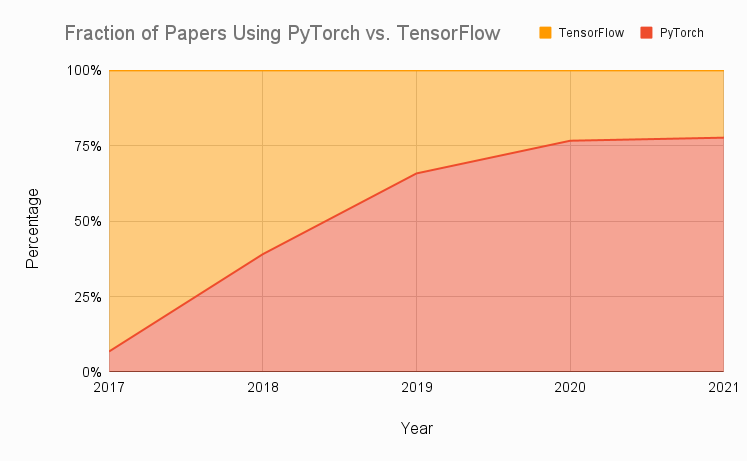
\includegraphics[width=\linewidth]{pytorch-1.png}
\caption{PyTorch, the state-of-the-art Deep Learning framework for Python.}
\label{fig:pytorch-sota}
\end{figure}

\note{\tiny My choice over the deep learning framework was not at random. Pytorch has both the best performance and the greatest outreach in the research community. In this figure, we can observe that it's main rival, Tensorflow, has experienced a decay over the years. That is mainly due to the capabilities of one over the other. Pytorch is better in terms of speed, rapid prototyping and debugging. Therefore, it is the framework that I chose to study as my point of reference for this project.}

\end{frame}

\section{Challenges}
\begin{frame}[fragile]{Numeric Nightmare (I)}

\begin{lstlisting}[language=Python]
>> 1234567890 + 0.000000001

ans =

    1.234567890000000e+09

>> eps

ans =

    2.220446049250313e-16

>> 
\end{lstlisting}

\note{\tiny We are going to elaborate now on the problems that an engineer is required to solve when implementing such applications. Let's start with this example. How much is one billion plus one to the power of minus 10? An uninitiated would answer a billion point 9 zeros and 1. But people like us must know that this sum is equal to one billion. Therefore, you can't just keep adding and multiplying numbers because the sum will eventually become huge. And you are going to run to overflow errors. The maximum value of an image in the dataset is 255. Can that be reduced? The answer is yes. We can use well known normalization methods and scale our data to belong between 0 and 1.}


\end{frame}

\begin{frame}[fragile]{Numeric Nightmare (II)}
\begin{lstlisting}[language=Python]
>> digits(30);
>> f = exp(sqrt(sym(163))*sym(pi));
>> vpa(f)
 
ans =
 
    262537412640768743.999999999999
 
>> 
\end{lstlisting}

\note{\tiny Our operations are all defined in the Real Numbers set. That means that we are dealing with floating points. Floating points in theory offer us a way to representing quantities with infinite numerical precision. However, in practice floating point numbers are nothing but a nightmare. How are you going to back-propagate the model error if you cannot accurately represent it? The answer is that you can't. To be able to do so, you would have to have an infinite memory, and that is not happening any time near. In fact the problem of the vanishing gradient is a well known issue when it comes to neural networks.}

\end{frame}

\begin{frame}{Numeric Nightmare (III)}
\begin{figure}
\centering
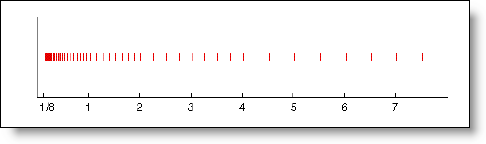
\includegraphics[width=\linewidth]{floatingCleve.png}
\caption{The nightmare of floating point arithmetic.}
\end{figure}

\note{\tiny But what's even worse than that? How can you protect your model from another well known numerical issue called underflow? First of all, you have to be prepared for such a problem. But of course when this is your first project, you don't foresee problems like that. And here I did have that problem. And it took me a week to find it. You see the sigmoid function here depends on the $\epsilon$ constant to perform forward propagation.}

\end{frame}


\begin{frame}{Numeric Nightmare (IV)}
\begin{figure}
\centering
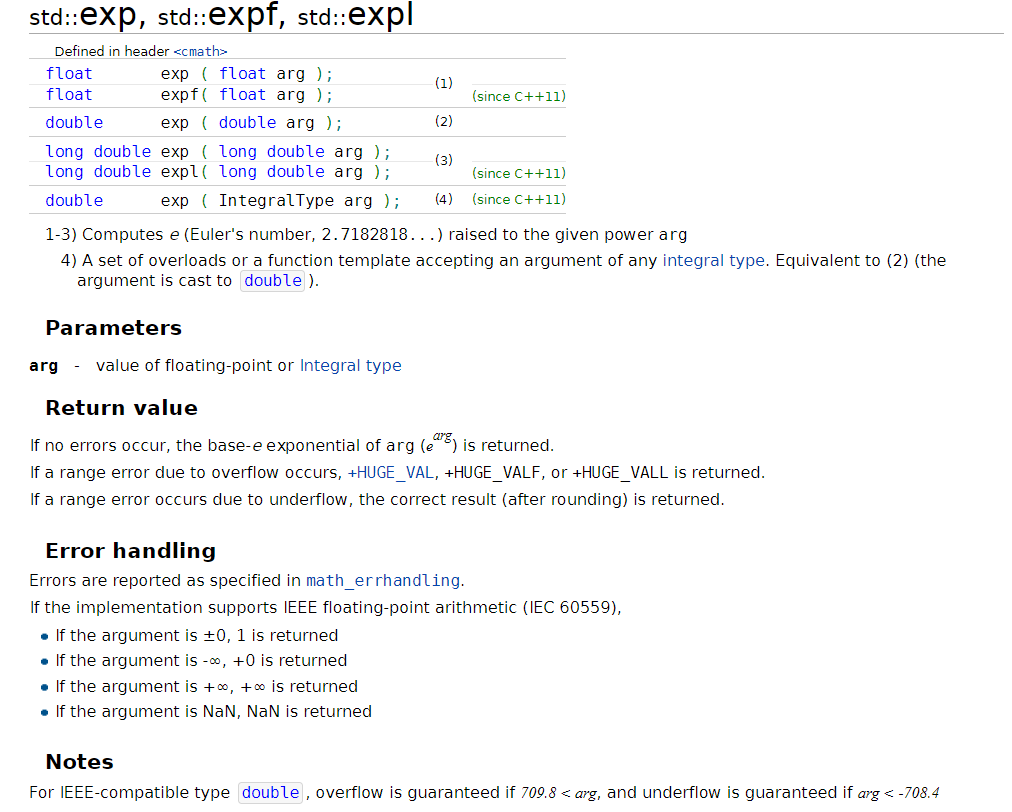
\includegraphics[height=0.8\textheight]{exp.PNG}
\caption{The \texttt{std::exp()} function.}
\end{figure}

\note{\tiny Let's therefore have a closer look at the provided \texttt{exp} function. And once you see it you know that you are in a bad situation. What is this in the notes section down? overflow is guaranteed if $709.8 < arg$, and underflow is guaranteed if $arg < -708.4$. Nice ah? For this purpose there are some very handy mathematical infinite series, called Taylor series.}

\end{frame}


\begin{frame}{Numeric Nightmare (V)}
\begin{tcolorbox}[colback=bg-block,colframe=second-fg-block,coltext=text-f,coltitle=title-block, title=The exponential function]
$
e^x \; = \; \sum_{n \, = \, 0}^{\infty} \frac{x^n}{n!} \; = \; 1 \; + \; \frac{x^2}{2!} \; + \; \frac{x^3}{3!} \; + \; \dots
$ 
\end{tcolorbox}

\note{Here you can see how to compute the exponential using a special subset of the Taylor series called Maclaurin series.}

\end{frame}

%%%%%%%%%%%%%%%%%%%% EXPERIMENTS %%%%%%%%%%%%%%%%%%%%
\section{Experiments}

\begin{frame}{The PyTorch model}
\begin{figure}
\centering
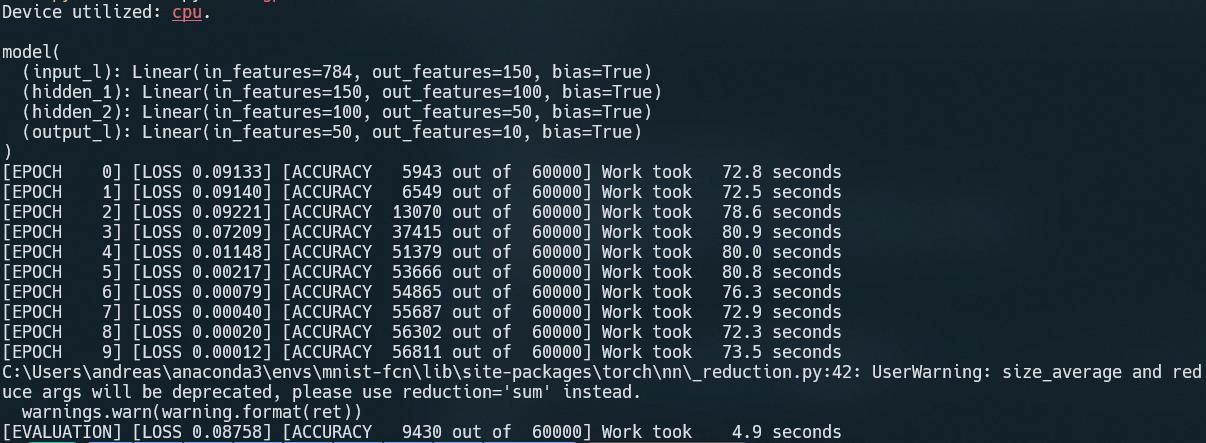
\includegraphics[width=\textwidth]{python-bench.PNG}
\caption{The PyTorch model.}
\label{fig:python-model}
\end{figure}

\note{\tiny Now to the exiting part, seeing the project actually working. First of all, let us see how did the PyTorch model go. This is 72 seconds per epoch. At this point, I would like to mention that Pytorch has actually some utilities that are connected which OneAPI and MPI all which optimize and parallelize the load of the model. So all I'm saying is that this is a fair fight. I'm not comparing my work with a frameworks that runs serial.}

\end{frame}

\begin{frame}{The serial C++ model}
\begin{figure}
\centering
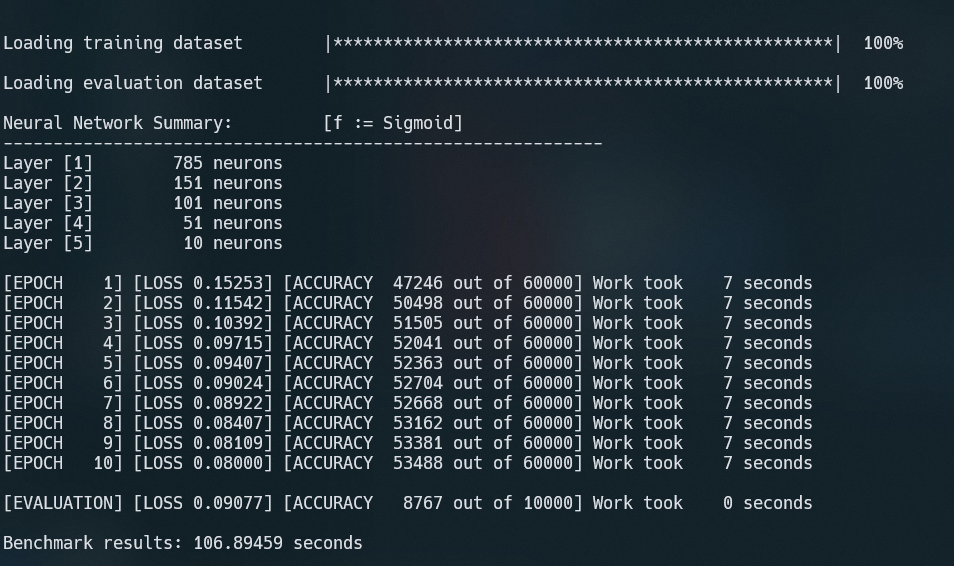
\includegraphics[width=\textwidth]{cpp-serial.PNG}
\caption{The serial $C$ $++$ model.}
\label{fig:cpp-serial-model}
\end{figure}

\note{Wow ... what happened here? 72 seconds per epoch down to 7 seconds per epoch. Ok ... that's going well! Can we go better?}

\end{frame}

\begin{frame}{The parallel C++ model}
\begin{figure}
\centering
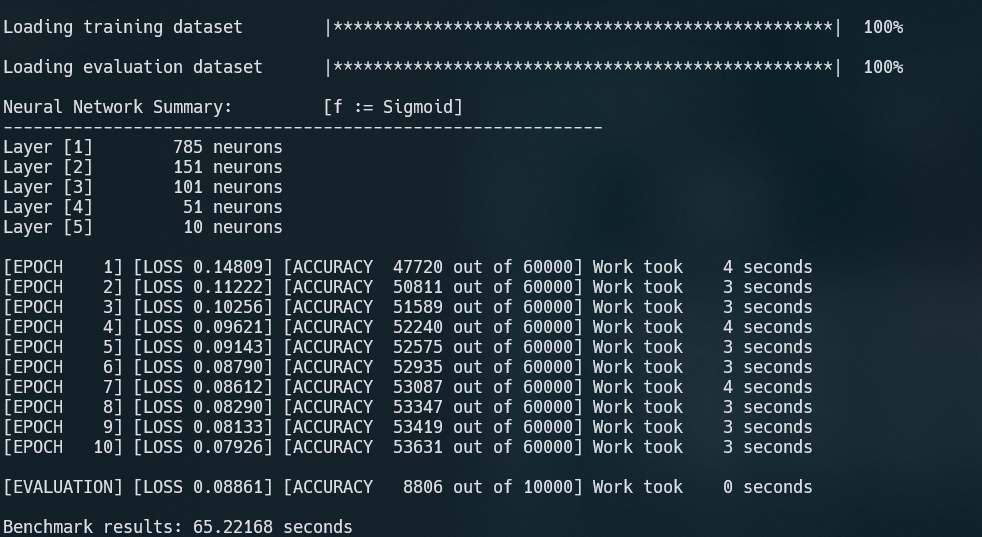
\includegraphics[width=\textwidth]{cpp-parallel.PNG}
\caption{The parallel $C$ $++$ model.}
\label{fig:cpp-parallel-model}
\end{figure}

\note{Apparently we can! So let's recap. From 72 seconds, down to 7 and then down to 3 ... That means that we achieved over 20 times performance boost. What does the profiler have to say about that?}

\end{frame}

\begin{frame}{Congrats, signed by Intel}
\begin{figure}
\centering
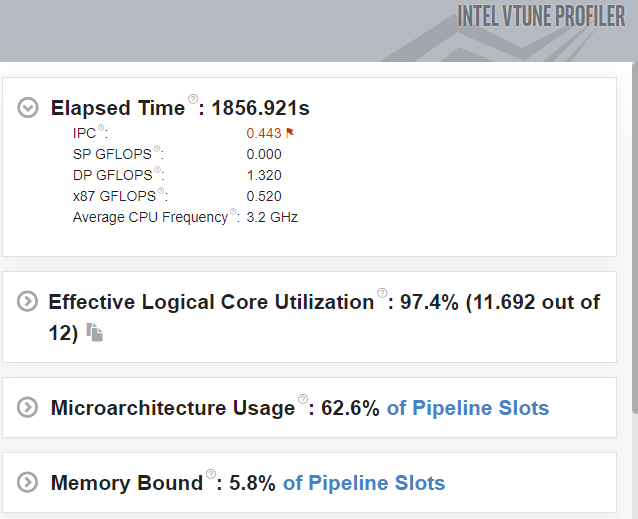
\includegraphics[height=0.8\textheight]{vtune.PNG}
\caption{The profiler report.}
\label{fig:profiler-report}
\end{figure}

\note{And this basically means that our application is not memory bound and has an effective core utilization percentage of approximately 98 percent.}

\end{frame}

%%%%%%%%%%%%%%%%%%%% APPENDICES %%%%%%%%%%%%%%%%%%%%
\appendix

{%
\usebackgroundtemplate{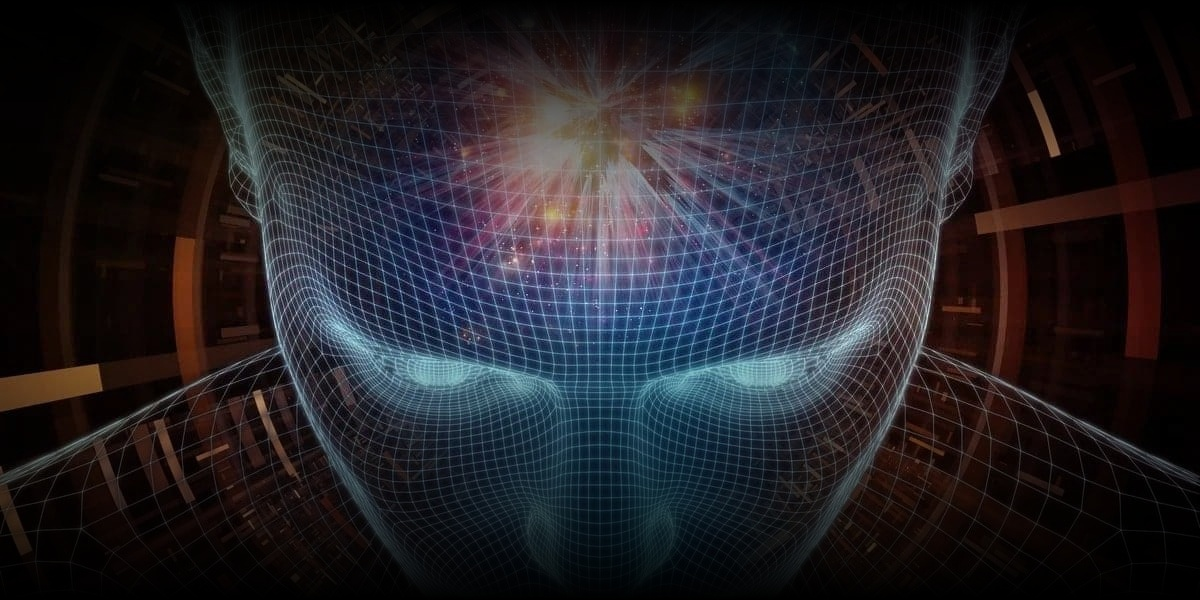
\includegraphics[width=\paperwidth, height=\paperheight]{cvBlurredOutput.jpg}}%
\begin{frame}{Thanks for your patience and time !}
\centering
\vspace*{5cm}
\Huge \color{fourth-fg-block} Questions (?)
\end{frame}
}

\end{document}


